\section{Results}
\label{sec:results}

\subsection{Regular regime ($\Re=45$): sample efficiency}
\label{sec:re45}

At $\Re=45$, GPPO reaches PPO's best 500-episode smoothed reward in
substantially fewer episodes in 4 of 5 seeds ($\text{seed}=0$:
\SI{63}{\percent} fewer; $\text{seed}=1$: $\sim$\SI{78}{\percent};
$\text{seed}=3$: $\sim$\SI{84}{\percent}; $\text{seed}=4$:
$\sim$\SI{70}{\percent}), and by a smaller margin at $\text{seed}=2$
($\sim$\SI{26}{\percent}). The \emph{direction} of GPPO's advantage over PPO
holds in all five seeds, and the $\text{seed}=0$ value (\SI{63}{\percent}) is
close to the paper's reported \SI{65}{\percent}~\cite{hydrogym2026} ---
evidence that our reimplementation captures the paper's mechanism.
\Cref{fig:re45curves} shows the seed-averaged learning curves.

\begin{figure}[t]
\centering
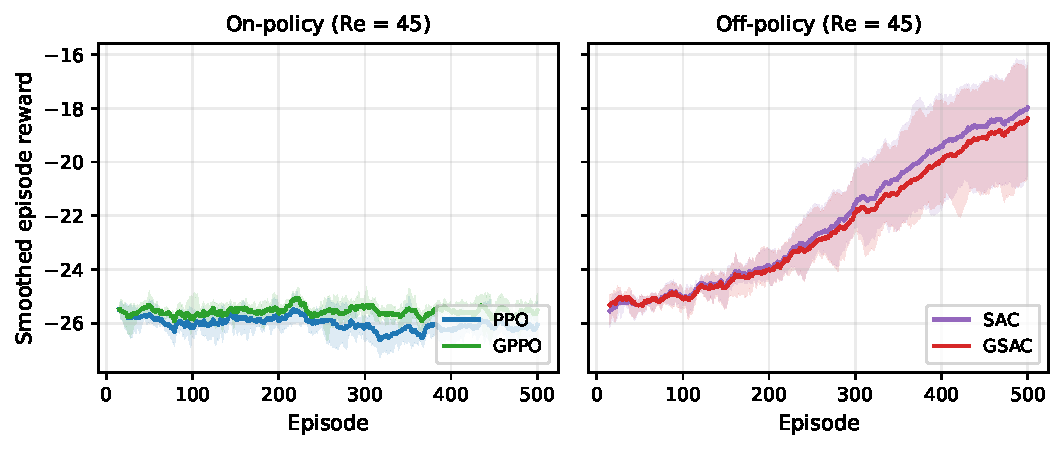
\includegraphics[width=\linewidth]{fig_re45_curves.pdf}
\caption{Regular regime ($\Re=45$). Seed-averaged smoothed episode reward
(15-episode window); shaded band is the seed-wise min--max envelope over the
five seeds. The off-policy family (right) converges to a markedly higher
reward level than the on-policy family (left); within each family the
analytic-gradient variant tracks its base algorithm closely.}
\label{fig:re45curves}
\end{figure}

\begin{figure}[tbp]
\centering
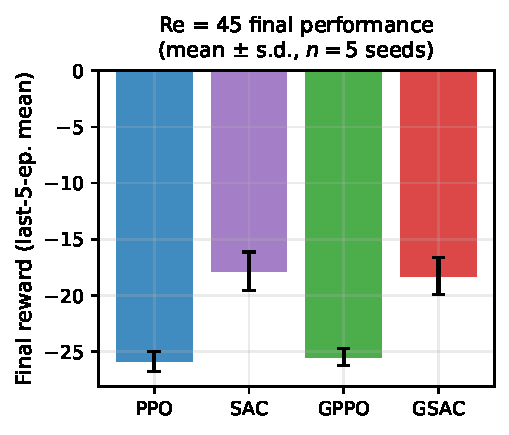
\includegraphics[width=0.6\linewidth]{fig_re45_final.pdf}
\caption{Final reward at $\Re=45$ (last-5-episode mean, mean $\pm$ s.d.\ over
five seeds). SAC/GSAC clearly outperform PPO/GPPO; GSAC does not exceed SAC.}
\label{fig:re45final}
\end{figure}

Two $\Re=45$ findings are seed-stable (\cref{fig:re45final}): (i) the
off-policy family reaches clearly better final reward than the on-policy
family in every seed --- its replay-buffer structure is already far more
sample-efficient, so no GPPO-style acceleration analysis applies to it; and
(ii) GSAC does not exceed SAC's final performance in any seed --- the
analytic gradient does not help the off-policy method in the regular regime.

\begin{table}[tbp]
\centering
\caption{Final performance at $\Re=45$, last-5-episode mean reward
(seed $=0\,/\,1\,/\,2\,/\,3\,/\,4$).}
\label{tab:re45}
\small
\begin{tabular}{|l|l|}
\hline
Algorithm & Final reward \\
\hline
PPO  & $-25.1\,/\,{-25.2}\,/\,{-27.2}\,/\,{-26.4}\,/\,{-25.6}$ \\
\hline
GPPO & $-25.4\,/\,{-24.6}\,/\,{-26.7}\,/\,{-25.4}\,/\,{-25.4}$ \\
\hline
SAC  & $-16.7\,/\,{-16.9}\,/\,{-18.9}\,/\,{-16.3}\,/\,{-20.3}$ \\
\hline
GSAC & $-18.0\,/\,{-17.1}\,/\,{-20.4}\,/\,{-16.3}\,/\,{-19.5}$ \\
\hline
\end{tabular}
\end{table}

\Cref{tab:re45} gives the exact per-seed values underlying \cref{fig:re45final}.
$\text{seed}=2$ trained to a worse level across all four algorithms, but the
\emph{relative} ordering is unchanged.

\subsection{Chaotic regime ($\Re=300$): the breaking point has no stable ordering}
\label{sec:re300}

In the chaotic regime all four algorithms have a breaking point ---
none completes 500 episodes stably; all eventually diverge (NaN)
(\cref{fig:re300curves}). The episode at which the break first occurs varies
by algorithm, but far more so \emph{by seed}: the ranking permutes across the
five seeds (\cref{fig:breakpoint}, \cref{tab:breakpoint}).

\begin{figure}[t]
\centering
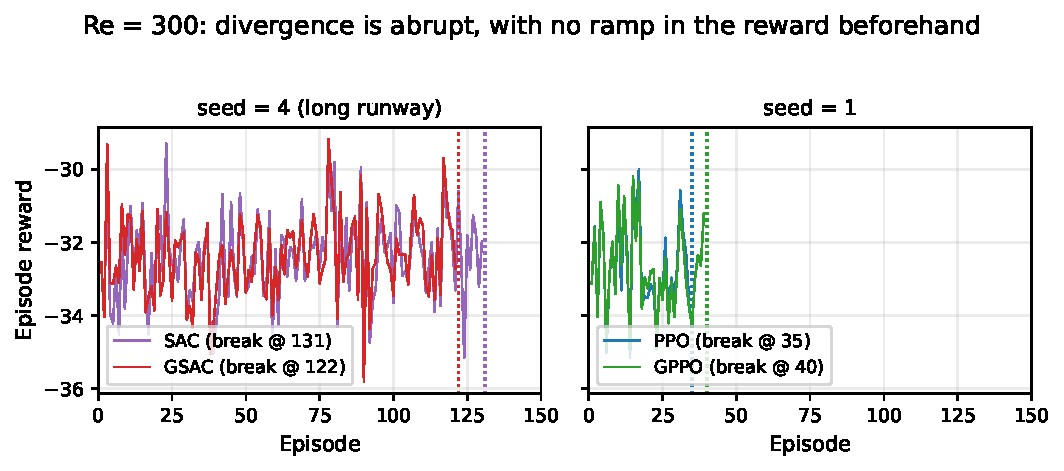
\includegraphics[width=\linewidth]{fig_re300_curves.pdf}
\caption{Example $\Re=300$ training curves. Left: the two long-runway
$\text{seed}=4$ off-policy runs (SAC breaks at episode 131, GSAC at 122).
Right: the $\text{seed}=1$ on-policy runs (PPO at 35, GPPO at 40). In every
case the reward is stationary until a single episode at which it collapses;
the dotted line marks the first-NaN episode.}
\label{fig:re300curves}
\end{figure}

The episode at which this collapse occurs is summarized across all seeds and
algorithms in \cref{fig:breakpoint}.

\begin{figure}[t]
\centering
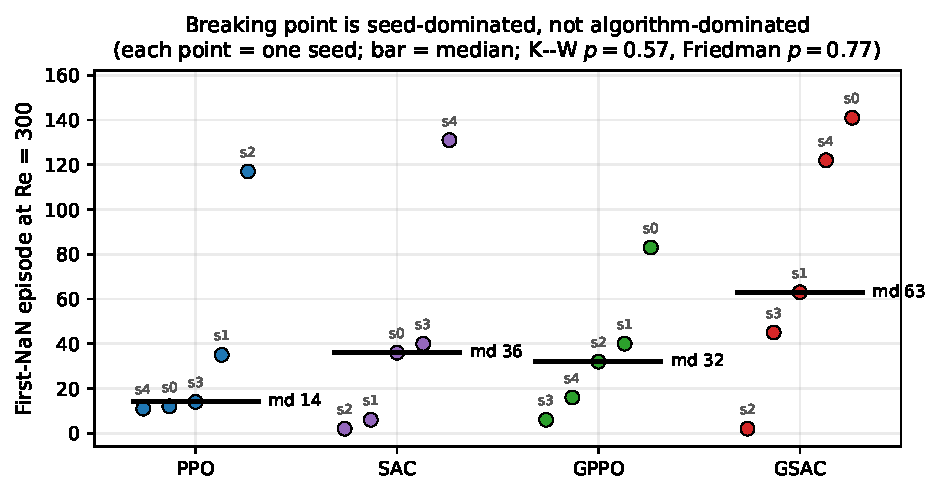
\includegraphics[width=0.86\linewidth]{fig_re300_breakpoint.pdf}
\caption{First-NaN episode at $\Re=300$: each point is one seed, the
horizontal bar is the per-algorithm median. Every algorithm's range spans
more than an order of magnitude, the medians overlap heavily, and no
omnibus test detects an algorithm effect (Kruskal--Wallis $p=0.57$, Friedman
$p=0.77$). GSAC has the highest median but is tied-last at $\text{seed}=2$.}
\label{fig:breakpoint}
\end{figure}

\Cref{tab:breakpoint} lists the exact per-seed episode counts underlying
this figure, together with the per-seed most-robust algorithm.

\begin{table}[t]
\centering
\caption{First-NaN episode at $\Re=300$ across the five seeds, with
per-algorithm median and mean. ``Most robust'' $=$ latest break in that seed.}
\label{tab:breakpoint}
\small
\begin{tabular}{|l|c|c|c|c|c|c|c|}
\hline
Algorithm & seed$=0$ & seed$=1$ & seed$=2$ & seed$=3$ & seed$=4$ & median & mean \\
\hline
PPO  & 12  & 35 & 117 & 14 & 11  & 14 & 37.8 \\
\hline
SAC  & 36  & 6  & 2   & 40 & 131 & 36 & 43.0 \\
\hline
GPPO & 83  & 40 & 32  & 6  & 16  & 32 & 35.4 \\
\hline
GSAC & 141 & 63 & 2 & 45 & 122 & 63 & 74.6 \\
\hline
most robust & GSAC & GSAC & PPO & GSAC & SAC & --- & --- \\
\hline
\end{tabular}
\end{table}

At $n=2$ (the conference version) two claims survived: analytic-gradient
injection delays the break (GPPO $>$ PPO, GSAC $>$ SAC) in direction, and
GSAC is the most robust of the four. At $n=5$ neither is a
statistically separable ordering.

Analytic-gradient injection does not delay the on-policy break: GPPO $>$
PPO holds at seeds 0, 1, 4 (83 vs 12; 40 vs 35; 16 vs 11) but
reverses hard at $\text{seed}=2$ (32 vs 117) and $\text{seed}=3$ (6 vs 14,
GPPO breaking first of all four). The paired per-seed difference GPPO$-$PPO
is $\{+71,+5,-85,-8,+5\}$, mean $\mathbf{-2.4}$ episodes, sign-flip
permutation $p=\mathbf{0.81}$.

GSAC leads by median but not significantly: its breaking point (median 63,
mean 74.6) is the highest of the four; it
is the most robust algorithm at seeds 0, 1, 3, second at $\text{seed}=4$, and
tied-last at $\text{seed}=2$ (the early-init failure mode of
\cref{sec:earlyinit} --- the flow diverges before learning begins and bare
SAC fails identically at the same episode). But the spread is enormous:
GSAC$-$SAC per seed is $\{+105,+57,0,+5,-9\}$, $p=0.38$; GSAC$-$GPPO is
$\{+58,+23,-30,+39,+106\}$, $p=0.19$; GSAC$-$PPO $p=0.38$.

What does hold across all five seeds are three seed-stable statements. Every algorithm eventually diverges at
$\Re=300$: analytic-gradient injection never prevents the break, it at most
postpones it. The break is never preceded by a visible precursor in the
reward or gradient signal (\cref{sec:precursor}). And the breaking point is
dominated by the seed --- within-algorithm variance across seeds (s.d.\
30--57 episodes) swamps the between-algorithm differences in mean (spread of
means 35--75). The ``clean multiplicative'' structure reported at $n=1$ and the ``GSAC most
robust'' claim that survived $n=2$ are both artifacts of small $n$. GSAC
carries a non-significant robustness lean --- highest median, most robust in
3/5 --- reported as a candidate effect, not a claim.

\subsection{Significance test ($n=5$)}
\label{sec:sig}

\Cref{tab:sig} gives the full pairwise comparison.

\begin{table}[t]
\centering
\caption{Pairwise breaking-point comparison at $\Re=300$, $n=5$. Exact
sign-flip permutation $p$ (two-sided); bootstrap \SI{95}{\percent} CI for the
median difference.}
\label{tab:sig}
\small
\begin{tabular}{|l|c|c|c|c|c|}
\hline
Comparison & per-seed diff (s0--s4) & mean & median & \SI{95}{\percent} CI (median) & $p$ \\
\hline
GPPO $-$ PPO  & $+71,+5,-85,-8,+5$      & $-2.4$  & $+5$  & $[-85,+71]$   & 0.81 \\
\hline
GSAC $-$ SAC  & $+105,+57,0,+5,-9$      & $+31.6$ & $+5$  & $[-9,+105]$   & 0.38 \\
\hline
GSAC $-$ GPPO & $+58,+23,-30,+39,+106$  & $+39.2$ & $+39$ & $[-30,+106]$  & 0.19 \\
\hline
GSAC $-$ PPO  & $+129,+28,-115,+31,+111$& $+36.8$ & $+31$ & $[-115,+129]$ & 0.38 \\
\hline
SAC $-$ PPO   & $+24,-29,-115,+26,+120$ & $+5.2$  & $+24$ & $[-115,+120]$ & 0.88 \\
\hline
GPPO $-$ SAC  & $+47,+34,+30,-34,-115$  & $-7.6$  & $+30$ & $[-115,+47]$  & 0.88 \\
\hline
\end{tabular}
\end{table}

Omnibus: Kruskal--Wallis $H=2.00$, $p=0.57$; Friedman $\chi^2=1.80$,
$p=0.77$. No pairwise or omnibus comparison reaches $p<0.05$. Per
the pre-registered decision rule (\cref{sec:intro}), the finding stands as
no statistically separable ordering of chaotic-regime training
stability by algorithm. GSAC's non-significant lean (highest median and
mean, most robust in 3/5 seeds, all pairwise $p\in[0.19,0.38]$) is reported
as a candidate effect for a future larger-$n$ study.

\subsection{Analytic-gradient norm}
\label{sec:gradnorm}

\Cref{fig:gradnorm} plots the analytic-gradient norm $\lVert\gan\rVert$ over
training, up to the break, for GPPO and GSAC in both regimes. Contrary to the
pre-registered hypothesis, $\lVert\gan\rVert$ does \emph{not} blow up before
the break at $\Re=300$: it fluctuates in the same $\sim$20--70 band as at
$\Re=45$ and shows no upward trend approaching the divergence episode. The
instability that ends training is therefore not visible in the gradient
magnitude --- a point developed mechanistically in \cref{sec:mechanism}.

\begin{figure}[t]
\centering
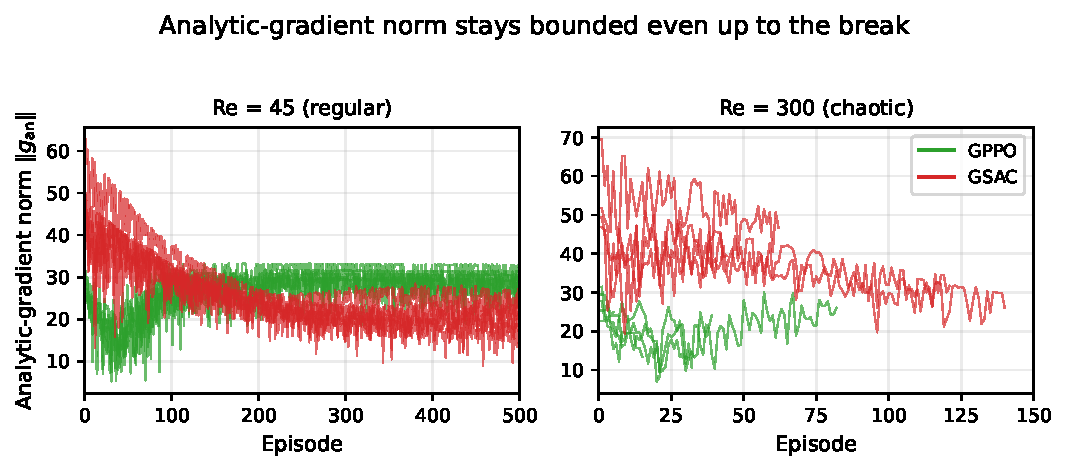
\includegraphics[width=\linewidth]{fig_gradnorm.pdf}
\caption{Analytic-gradient norm $\lVert\gan\rVert$ per episode (all five
seeds overlaid), truncated at each run's first-NaN episode. Left: $\Re=45$.
Right: $\Re=300$. The norm stays bounded and trend-free right up to the
break; the chaotic-regime divergence is not preceded by a gradient
explosion.}
\label{fig:gradnorm}
\end{figure}
